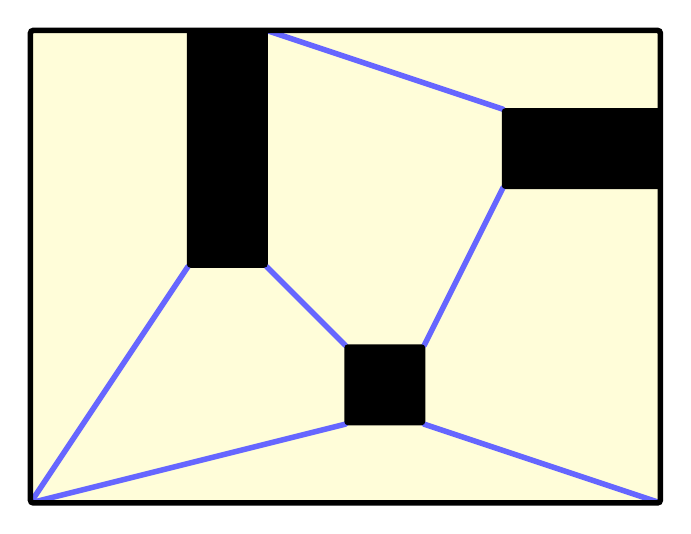
\begin{tikzpicture}[thick,scale=1, every node/.style={scale=0.8}]

\begin{scope}

\clip (0,0) -- (8,0) -- (8,-6) -- (0,-6) -- cycle;

\draw [line width=0,fill=yellow!15!white] (0,0) -- (8,0) -- (8,-6) -- (0,-6) -- cycle;

\draw [blue!60!white,line width=2,line cap=round] (3,0) -- (6,-1);

\draw [blue!60!white,line width=2,line cap=round] (5,-4) -- (6,-2);

\draw [blue!60!white,line width=2,line cap=round] (2,-3) -- (0,-6);

\draw [blue!60!white,line width=2,line cap=round] (3,-3) -- (4,-4);

\draw [blue!60!white,line width=2,line cap=round] (4,-5) -- (0,-6);

\draw [blue!60!white,line width=2,line cap=round] (5,-5) -- (8,-6);

\draw [fill=black,rounded corners=1] (2,0) -- (3,0) -- (3,-3) -- (2,-3) -- cycle;

\draw [fill=black,rounded corners=1] (6,-1) -- (8,-1) -- (8,-2) -- (6,-2) -- cycle;

\draw [fill=black,rounded corners=1] (4,-4) -- (5,-4) -- (5,-5) -- (4,-5) -- cycle;

\end{scope}

\draw [line width=2,rounded corners=1] (0,0) -- (8,0) -- (8,-6) -- (0,-6) -- cycle;

\end{tikzpicture}